\chapter{Continuous-wave lineal frequency modulation (CWLFM) radars for gait analysis}
\chaptermark{CWLFM radars for gait analysis}

It has been shown in \cref{cha:generalities} that the most promising method for gait analysis involves the use of continuous-wave lineal frequency modulation (CWLFM) radars. Employing a single radar or a network of radars to analyse gait and extract useful information has been proved accurate and robust to other factors that could hinder the data extraction from the signals, compared to other methods. For that matter, it has been shown that current radar solutions require voluminous, expensive and inefficient hardware that is not scalable and easy to deploy in real-life scenarios, should the gait of a patient be analysed.

Moreover, the current system proposals are designed exclusively to work with one radar node. State-of-the-art research is now focused on implementations that feature a multi-static radar network, composed of several radar nodes, positioned in different locations that ---by working synchronously--- can extract data simultaneously, and by processing the netted radar signals, the extraction of more accurate and useful information for gait analysis is achieved [REF ZZZ]. The current design described in \cref{cha:generalities} is not suitable to support the configuration of a radar network of multiple nodes due to the high-cost and amount of space required by the system. It is of interest to design a new radar system pipeline that can be adapted to work in a multi-static radar network. In this chapter, the radar and communication requirements specific to gait analysis are analysed. After analysing the requirements of the application, a new radar node design is described, which addresses the problems of current implementations, focusing on compactness, energy-efficiency, cost-efficiency and ability to be adapted to work in a multi-static radar network.

\section{Radar and communications requirements}

To understand the characteristics of the radar signal used for gait analysis, it is important to fix the radar parameters that enable gait analysis in a particular scenario. For the purposes of this Bachelor's Thesis, and aligned to the common application of CWLFM radars for gait analysis [REF ZZZ], an indoor scenario and a target of a human being is considered. In this section, the resulting radar operating conditions are described.

Moreover, the signals generated at the input of the voltage-controlled oscillator (VCO), the output trigger signals and the output intermediate frequency (IF) signals in the baseband board are characterised to understand the operation of the radar.

\subsection{Radar parameters}

From the context of gait analysis and following from \cref{eq:fs_final}, it is possible to obtain radar parameters that correspond to this context of operation. In \cref{eq:fs_final}, $R_{\max}$ and $\nu_{r\max}$ are constants that depend on the environment and the case of radar use. In this context of measuring the gait of a person, the environment is indoors and the target is a walking human being. The target linear velocity should be around $\SI{5}{\kilo\meter\per\hour} \approx \SI{1.4}{\meter\per\second}$. The goal is to obtain measurements from moving parts of the body. The fastest moving parts are the arms, which have a maximum radial velocity of around \SI{3}{\meter\per\second}. Therefore, $\nu_{r\max} = 1.4 + 3 = \SI{4.4}{\meter\per\second}$. A margin of error is left to avoid measurement errors from sudden movements of body parts. Thus, $\nu_{r\max} =\SI{5.9}{\meter\per\second}$.

With these constraints, it is possible to obtain the minimum sampling frequencies and the maximum pulse repetition intervals for radars with different bandwidths and working frequencies by solving \cref{eq:fs_final}. A series of examples are shown in \cref{tab:fs_Tc}.

\begin{longtable}{@{}cccc@{}}
	\toprule
	$\mathbf{f_0}$ \textbf{(GHz)}& $\mathbf{W}$ \textbf{(GHz)} & $\mathbf{f_{s\min}} \textbf{(MHz)}$& $\mathbf{T_c}$ \textbf{(\si{\micro\second})} \\* \midrule
	\endhead
	24.0 & 2.0 & 0.5 & 529.7 \\
	24.0 & 4.0 & 1.0 & 529.7 \\
	24.0 & 5.0 & 1.3 & 529.7 \\
	66.0 & 4.0 & 2.8 & 192.6 \\
	134.0 & 1.0 & 1.4 & 94.9 \\* \bottomrule
	\caption{Sampling frequencies and pulse repetition intervals for different parameters.}
	\label{tab:fs_Tc}
\end{longtable}
	\change[inline]{no me convence esta tabla, cambiar por un gráfico que relacione los distintos aspectos y resumen de lo que se habla en esta sección (en forma de esquema)}

\subsection{Radar operating conditions for gait analysis} \label{sec:radar_operating_conditions}

For the purpose of this Bachelor's Thesis, the measurement and operation of the system is carried out under the following conditions:
\begin{equation} \label{eq:if_conditions}
	f_0 = \SI{24}{\giga\hertz} \qquad W = \SI{2}{\giga\hertz} \qquad f_{s\min} = \SI{0.5}{\mega\hertz} \qquad T_c = \SI{525}{\micro\second}
\end{equation}

This yields the following maximum operating range ($R_{\max}$):
\begin{align}
	f_s c^2 &= 16 R_{\max}W f_0 \nu_{r\max} \\
	R_{\max} &= \frac{f_s c^2}{16 W f_0 \nu_{r\max}} = \SI{9.917}{\meter}
\end{align}
which is sufficient for an indoor environment of operation requiring around \SI{10}{\meter} distance maximum. The current radar node is configured with the obtained parameters of the CWLFM signal.

\subsection{Voltage ramp at the input of the voltage controlled oscillator}

As described in \cref{sec:cwlfm_wp}, CWFM radars sweep continuously a certain RF band. The MMIC used in the current radar node, TRX-024-046 \cite{ZZZ}, with the operating conditions described in \cref{sec:radar_operating_conditions}, sweeps the frequency band between \SI{23}{\giga\hertz} and \SI{25}{\giga\hertz}. The RF sweep is controlled by the VCO present in the baseband board. The voltage at its input is controlled with a phase-locked loop (PLL) as described in \cref{sec:baseband_general}.

During a sweep cycle the voltage at the input of the VCO increases constantly to cover the whole frequency band. The evolution of the voltage with time has the shape of a rising ramp, as it is shown in Figure ZZZ. At the end of the sweep cycle, the voltage at the input of the VCO decreases to begin another sweep cycle. To prevent the PLL from unlocking during a large period of time, at the end of the sweep cycle, the voltage at the input of the VCO decreases smoothly. The evolution of the voltage with time has the shape of a falling ramp steeper than the aforementioned rising ramp. This falling ramp is referred to as dual ramp.

The VCO ramps are measured with an Agilent MS ZZZ oscilloscope and the data is captured. Under the conditions described in \cref{sec:cwlfm_wp}, the rising ramp has a duration of \SI{505}{\micro\second}. The dual ramp has a duration of \SI{20}{\micro\second}. Thus, a complete sweep cycle has a duration of $T_c = \SI{525}{\micro\second}$. The voltage at the input of the VCO is shown in Figure ZZZ. Despite the dual ramp, the PLL unlocks for a short period of time at the beginning of the rising ramp. The state of the PLL during the ramp phases is shown in Figure ZZZ. 

\subsection{Trigger signals characterisation}

In addition to the IF signals, the baseband stage also outputs a trigger signal to allow the ADC in the acquisition stage to determine the beginning of each ramp of the signal. The trigger signal is measured in conjunction with the VCO ramps with an Agilent MS ZZZ oscilloscope and the data is captured. In Figure ZZZ, it is shown the measured ramps and trigger signal.

It can be seen that the trigger signal has a high value at the end of the rising ramp and and at the end of the dual ramp. It has a low value elsewhere. The characteristics of the trigger signal are shown in Table ZZZ.

\subsection{Intermediate frequency (IF) signals characterisation} \label{sec:if_signals_characterisation}

With the configuration described in \cref{sec:radar_operating_conditions}, the signals output by the baseband stage from the current radar node are characterised. From the characterisation, the most important aspect is the voltage range of the signal. As the sampling of these signals is later carried out by the acquisition stage, the input range of the acquisition stage must be compatible with the output voltage range of the IF signals from the baseband stage.

The radar is configured according to \cref{sec:radar_operating_conditions} and put in operation. The $I_\mathrm{rad}$ and $Q_\mathrm{rad}$ signals are then measured with an Agilent MS ZZZ oscilloscope and the data is captured. The measured ramp signals for one sweep cycle are shown in Figure ZZZ.

It can be seen that the voltage range of the IF signals from the baseband board have the following characteristics:
\begin{align} \label{eqn:iq_volts}
	I_\mathrm{rad}(t) &\in [-0.8, 0.8]\ \si{\volt} \\
	Q_\mathrm{rad}(t) &\in [-0.4, 0.4]\ \si{\volt}
\end{align}
The acquisition stage input range must contain these values, otherwise an additional conditioning stage must be developed to adequate the signals to the input range of the ADC in the acquisition stage.



% TODO: contar rising ramp, double ramp, pll unlocked



\section{New radar node design}

To address the problems related to the high-cost, non real-time operation and scalability of the current radar node, a new acquisition stage is designed. This design addresses the more expensive part of the current radar node, which is the acquisition stage, as shown in \cref{sec:hw_cost} and allows for the simultaneous capture of signals from different radar nodes. For this purpose the new acquisition stage principle involves the substitution of the high-cost, energy-inefficient and voluminous PC with ADC card configuration with a microcontroller unit (MCU). This new stage is designed in a printed circuit board (PCB) layout and manufactured accordingly. The MCU chosen is the STM32WB15CC MCU from ST Microelectronics \cite{STMicroelectronics2022} and the criteria based on its selection is described in this section.

Moreover, it is decided that the new acquisition stage must communicate and transmit the digital signals from the radar wirelessly. To benefit from low energy consumption, real-time transmission of data, minimal power requirements as well as ease of integration [REF], the Bluetooth Low Energy (BLE) protocol is chosen as the interface to transmit sampled data. This interface substitutes the physical connection of the ADC card to the PC via de PCI port. A receiving device equipped with Bluetooth capabilities receives the sampled data coming from the radar node to visualise and perform additional processing if needed. The characteristics of this wireless communication link and the criteria based on its selection is also described in this section.

The MCU present in the new acquisition stage handles the sampling of the signals using and embedded ADC, further lowering the cost as it is not necessary to include an external ADC component into the acquisition stage. Due to this fact, the embedded ADC input voltage range is different to the one of the current acquisition stage. As a consequence, an additional intermediate frequency (IF) stage has been designed to condition the signal to the operating range of the MCU ADC. The design of this IF stage is described in this section.


\subsection{Intermediate frequency (IF) signal characteristics}

Signal preprocessing is performed in this stage in order to allow the sampling by the MCU of the I-Q modulated incoming signal from the radar.

This stage is necessary because the MCU has an ADC whose operating voltage input range differs from that of the incoming signal, and the incoming signal is differential, while the sampling is performed from single-ended inputs. In their limit condition [REF],
\begin{equation} \label{eqn:iq_volts}
	I(t), Q(t) \in [-0.4, 0.4]\ \si{\volt}
\end{equation}
An example output of I and Q signals at this condition can be found in figure ZZ.

In this chapter, the limitations of the ADC, the proposed design to make the signal comply with its constraints, and the resulting acquisition and preprocessing stage are discussed.

\section{ADC1 limitations}

The chosen microcontroller unit has one integrated high-speed and general-purpose successive approximation (SAR) ADC, labelled ADC1. The sampling characteristics of ADC1, such as the input signal voltage and current bounds, as well as the maximum sampling rate, are important to account for the limitations of the acquisition system.

First, the input range of ADC1 is $[0, V_{DDA}]\ \si{\volt}$, with $V_{DDA}$ being the DC voltage supply of the analogue peripherals in the MCU.
\cite[p.~103]{STMicroelectronics2022}. The supply chosen for $V_{DDA}$ that complies with its general operating condition range \cite[p.~62]{STMicroelectronics2022} is \SI{3.3}{\volt}, resulting in an input range of $[0, 3.3]\ \si{\volt}$. This differs from the input signal range expressed in \cref{eqn:iq_volts}, so scaling and DC-shifting of the signal are necessary.

Moreover, the ADC has a limitation on the sampling rate depending on the bit resolution of the ADC samples and the supply voltage. With the chosen voltage supply of \SI{3.3}{\volt} and choosing the highest resolution available of \SI{12}{\bit}, the maximum sampling rate achievable is \SI{2.5}{\mega s\per\second} \cite[p.~103]{STMicroelectronics2022}.

Finally, ADC1 features 10 single-ended input channels that can be sampled sequentially \cite[p.~355]{STMicroelectronics2022a}. The system only makes use of the first two channels, Ch1 and Ch2, mapping the previously processed I signal to Ch1 and the Q signal to Ch2.

Since the channels are sequentially sampled and all information from both signals needs to be preserved, the limitations of the Nyquist-Shannon sampling theorem must then be met. Therefore,
\begin{equation} \label{eqn:nyquist_sampling}
	f_{s_{I}}, f_{s_{Q}} \ge 2 f_{i_{\max}}
\end{equation}

Given that ADC1 has a total sampling rate of \SI{2.5}{\mega s\per\second} \cite[p.~103]{STMicroelectronics2022}, every channel will be sampled at half the total sampling rate $2.5/2 = \SI{1.25}{\mega s\per\second}$. Thus,
\begin{equation} \label{eqn:nyquist_sampling}
	f_{I_{\max}}, f_{Q_{\max}} \le \frac{\SI{1.25}{\mega s\per\second}}{2} = \SI{625}{\kilo\hertz}
\end{equation}

This limits the system in such a way that the frequency of the IF signals coming from the radar system must be $ 0 \le f_i \le \SI{625}{\kilo\hertz}$.
% TODO: Write that this limitation is in accordance with targets located within a specific range of the radar (ask Nacho)

\section{Filtering step}
The incoming I-Q signals are filtered before the conditioning stage for two main reasons: to improve the SNR by reducing high-frequency noise and limiting the processed bandwidth to useful signal information and to convert a pair of differential signals to two single-ended signals.
\subsection{Filter design}
\change[inline]{Creo que no hay filtering, confirmar con Nacho}
\section{Signal conditioning step}
In this step, the single-ended filtered signals are modified according to the input constraints of ADC1. This involves amplifying the signal and shifting it by a positive DC offset.
\subsection{Signal conditioning design}
In order to drive the ADC correctly and minimise measurement errors, a careful design of the driving circuit is carried out. First, considering the internal SAR ADC sampling mechanism \cite[pp.~356,~363]{STMicroelectronics2022a}, the driving input to the ADC must have low impedance to benefit from a low gain error, low settling time error, and less distortion \cite{Franco2014}. This is achieved by driving the input with a non-inverting op-amp tailored to provide a specific gain and to offset the input by a reference voltage.

Parting from recommended ADC buffer design guidelines from Texas Instruments \cite[p.~17]{TexasInstruments2022}, the circuit is shown in \cref{fig:if_cir}.

\begin{figure}[h]
	\centering
	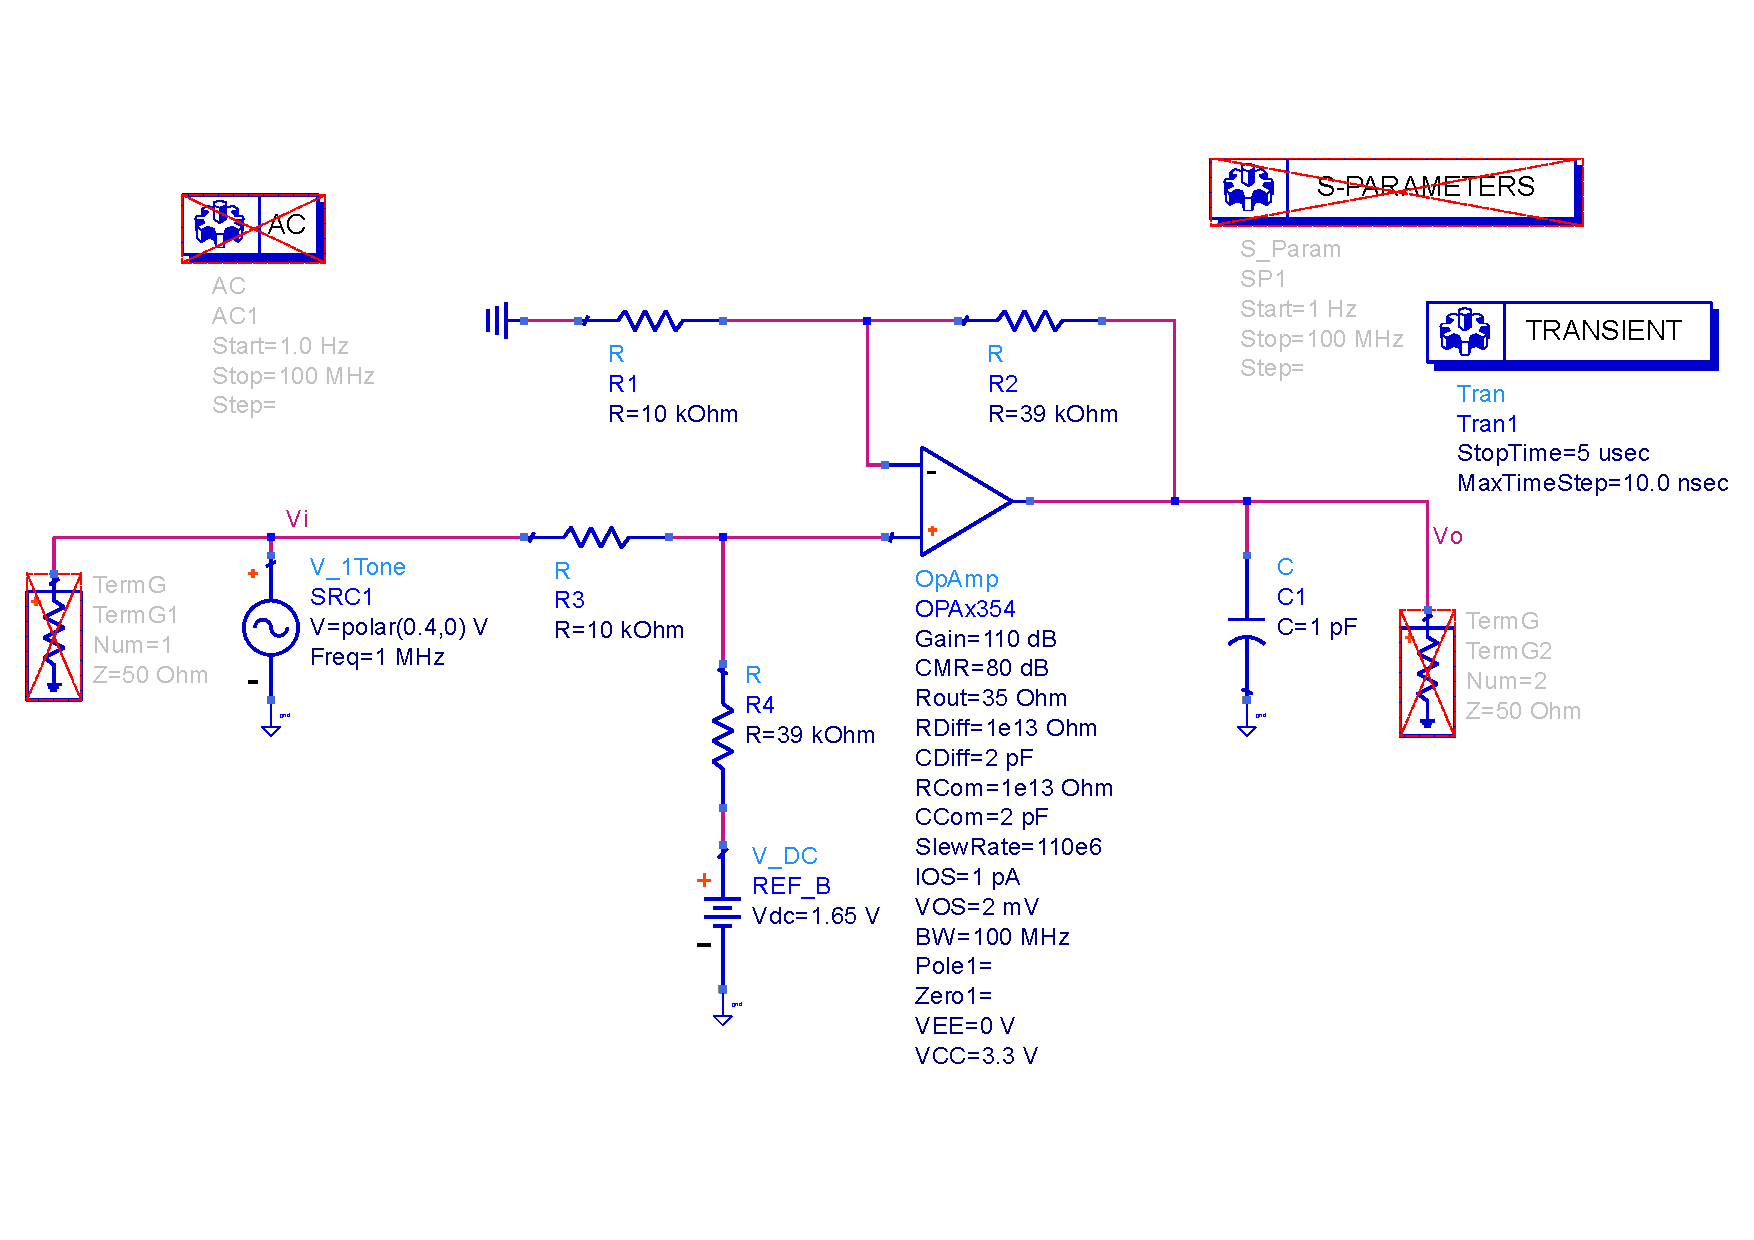
\includegraphics[width=\linewidth]{if_stage_sucio/prueba_impresion_ads.pdf}
	\caption{Circuit of the IF stage signal conditioning step}
	\label{fig:if_cir}
\end{figure}

The OA used in the driver can be any op-amp having a GBW that is able to accommodate all the incoming signal from the filter:
\begin{equation}
	GBW_{OA} \ge \frac{BW_{f}}{G}
\end{equation}
being $G$ the gain of the OA and $BW_{f}$ the bandwidth of the filter.


\subsubsection{Gain configuration}
The values of $R_1, R_2, R_3, R_4$ are responsible for setting the gain $G$ of the OA.
In this particular application a pure AC waveform of $0.8 Vpp$ needs to map to a waveform of $3.3 Vpp$, thus:
\begin{equation}
	G = \frac{3.3}{0.8} = 4.125
\end{equation}
and after analysing the circuit feedback loops:
\begin{gather}
	G = \frac{R_4}{R_1} \frac{R_1+R_2}{R_3+R_4}\\
	R_1 = R_3, R_2=R_4\\
	G= \frac{R_4}{R_1}
\end{gather}
after giving a fixed value of \SI{10}{\kilo\ohm} to $R_1$:
\begin{equation}
	G \cdot \SI{10}{\kilo\ohm} = R_4 = \SI{41.25}{\kilo\ohm}
\end{equation}
By allowing for some margin at the extrema of the output, and considering that there aren't commercial resistors of the computed value, the closest E12 value of \SI{39}{\kilo\ohm} has been chosen for $R_4$.
At the output of the OA, a small capacitor is placed in parallel to allow for smooth voltage output and high-frequency voltage spikes suppression.

%OA selection (el del laboratorio) formula de antes
\subsubsection{OA selection}
The chosen OA for the task has been OPA2354AIDDA [REF], because it has a sufficiently large bandwidth for the application (suitable GBW) and there is readily available stock at the laboratory.

\subsection{Signal conditioning simulation}

After obtaining all these parameters, the circuit is laid out in Keysight ADS, a circuit simulation software.

\subsubsection{Transient simulation}
The circuit is simulated at its limit conditions for both voltage and frequency. The simulation result can be found in the figures according to the following list:
\begin{description}
	\item [$f_{i_{\max}}, V_{\max}$] \cref{fig:fmax_vmax}
	\item [$f_{i_{\max}}, V_{\min}$] \cref{fig:fmax_vmin}
	\item [$f_{i_{\min}}, V_{\max}$] \cref{fig:fmin_vmax}
	\item [$f_{i_{\min}}, V_{\min}$] \cref{fig:fmin_vmin}
\end{description}

\todo[inline]{Faltan añadir: Vmin, fmax; Vmax, fmin; vmin, fmin y el ancho de banda de esta stage.}

The simulations conclude that the operation of the signal conditioning stage follows the constraints of the ADC1 input signals, and having a flat response for all the specified IF operating frequencies.

\begin{figure}[h]
	\centering
	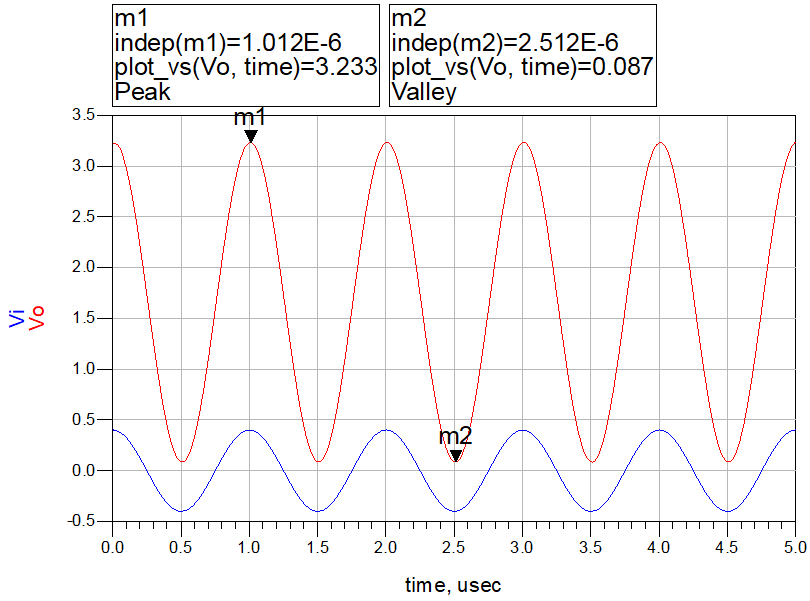
\includegraphics[width=\linewidth]{if_stage_sucio/1Mhz_transient.png}
	\caption{Transient simulation with an input at $f_{i_{\max}} = \SI{1}{\mega\hertz}$ and $V_{\max} = 0.8 Vpp$}
	\label{fig:fmax_vmax}
\end{figure}

\section{IF stage modular circuit design}
After all the simulations are performed and verified the circuit schematic is design following power distribution design for all the stages an following manufacturer guidelines of the different ICs used in the design. The obtained schematic can be seen in \cref{fig:if_sch}.

Two debug SMA connector have been installed in the transition from the filtering part to the signal conditioning part in order to check the correct operation of both parts independently. Moreover, a JTAG connector labelled (J\_AUX) has been added to provide and inspect the different power supplies of the circuit in testing.
\begin{figure}[h]
	\centering
	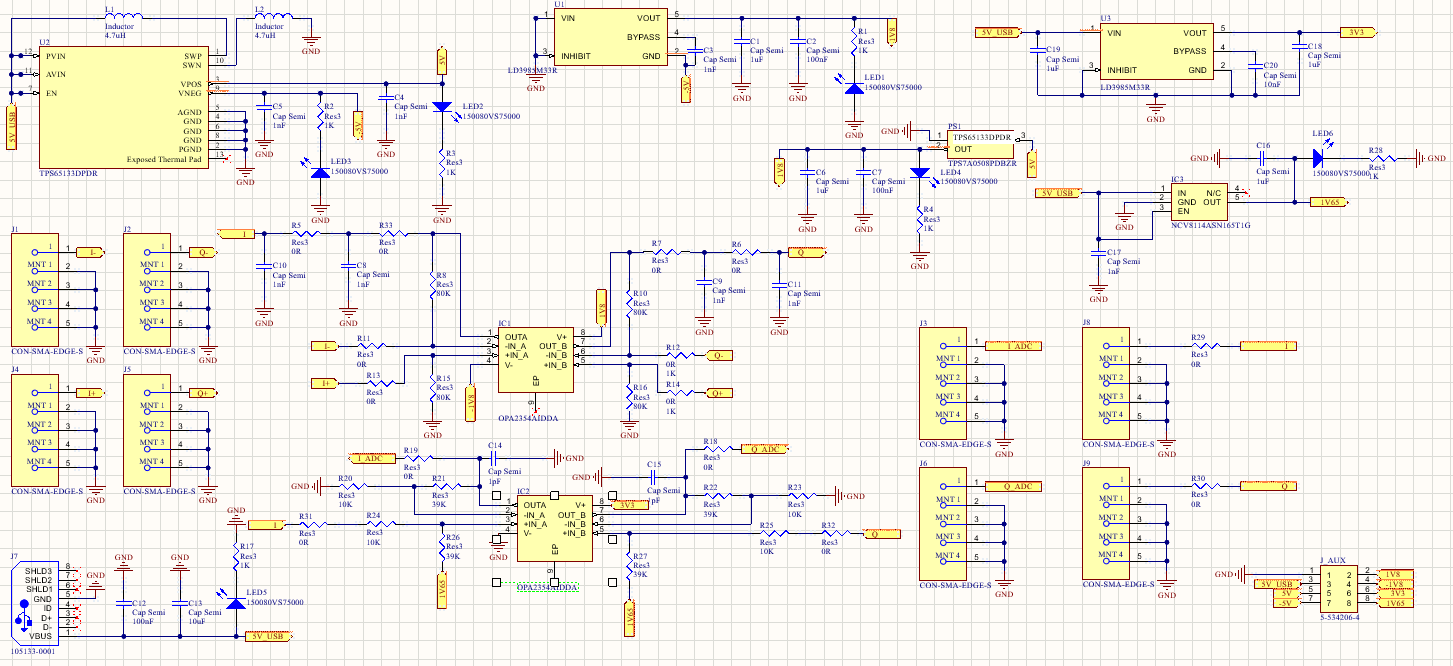
\includegraphics[width=\linewidth]{if_stage_sucio/if_sch.png}
	\caption{Circuit schematic of the IF stage}
	\label{fig:if_sch}
\end{figure}

%\subsection{Power distribution}
\subsection{Circuit integration and layout}
Finally, according to the schematic, the PCB layout is performed. Some considerations have been accounted for in this stage such as separating the filtering part and the signal conditioning part as much as possible and providing sufficient space between the power supply part, which features high-frequency switching power components, and the analog OA parts. The 5V base power supply is obtained from an USB connector plugged in to a 5V power brick. The resulting layout can be found in \cref{fig:if_layout}.

\begin{figure}[h]
	\centering
	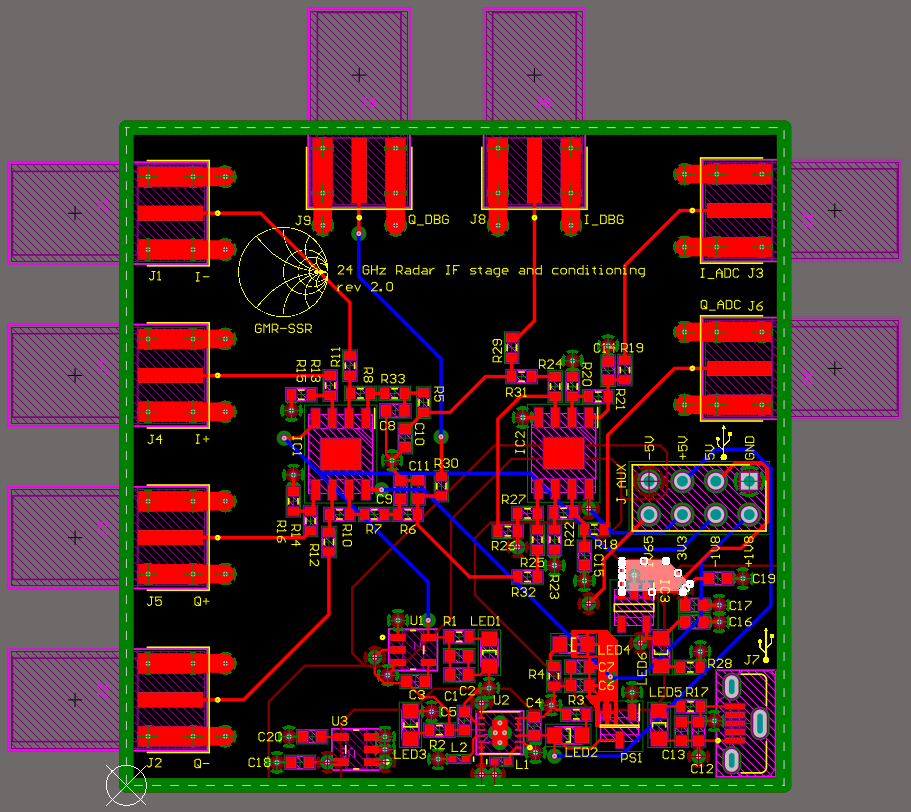
\includegraphics[width=\linewidth]{if_stage_sucio/layout.png}
	\caption{PCB layout of the IF stage}
	\label{fig:if_layout}
\end{figure}

The final PCB layout is sent to manufacturing, and after assembly and soldering of the ICs, the resulting PCB can be found in \cref{fig:if_phy}.

\begin{figure}[h]
	\centering
	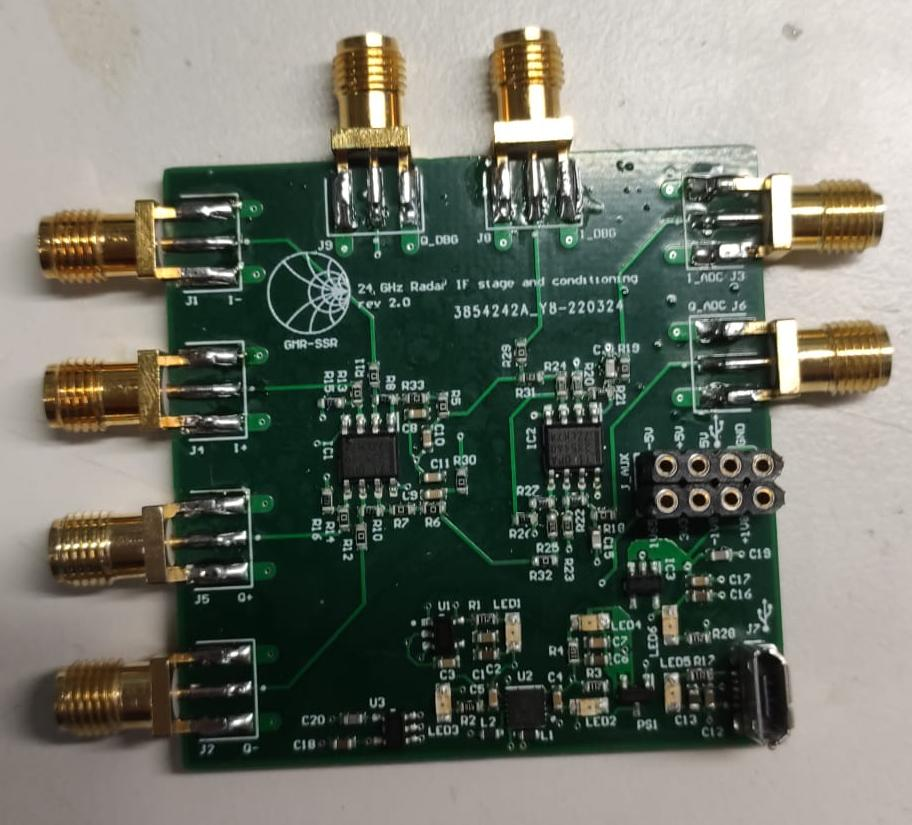
\includegraphics[width=\linewidth]{if_stage_sucio/if_phy.jpeg}
	\caption{Manufactured and assembled IF PCB}
	\label{fig:if_phy}
\end{figure}

\section{IF stage circuit testing}

\change[inline]{WIP: Insertar gráficas del csv del osciloscopio de las pruebas y explicar la obtención de resultado y el proceso de medida, poner como he hecho las medidas, REF al datasheet del osciloscopio y sampling rate del osciloscopio (procurar poner la misma)}


\subsection{Conditions of operation}
\change[inline]{Referencia a las condiciones de funcionamiento del radar y explicación de la elección de las condiciones a continuación}
For the purpose of this Bachelor's Thesis, the measurement and operation of the system is carried out under the following conditions:
\begin{equation} \label{eq:if_conditions}
	f_0 = \SI{24}{\giga\hertz} \qquad W = \SI{2}{\giga\hertz} \qquad f_{s\min} = \SI{0.5}{\mega\hertz} \qquad T_c = \SI{529.7}{\micro\second}
\end{equation}

This yields the following maximum operating range ($R_{\max}$):
\begin{align}
	f_s c^2 &= 16 R_{\max}W f_0 \nu_{r\max} \\
	R_{\max} &= \frac{f_s c^2}{16 W f_0 \nu_{r\max}} = \SI{9.917}{\meter}
\end{align}
which is sufficient for an indoor environment of operation requiring around \SI{10}{\meter} distance maximum.

\section{Hardware adaptation and development}
\todo[inline]{Principales desarrollos de la parte MCU e IF (redactar del documento if\_stage.docx), aquí detallar elección de MCU según constraints}
To digitise these signals without losing useful information it is decided to use a microcontroller unit (MCU) with an integrated ADC. The integrated ADC must have a sufficient sampling rate to avoid information loss when sampling as per \cref{eq:nyquist}. In the radar operation conditions, the minimum sampling frequency ($f_{s\min}$) required for the radar signals is given in \cref{eq:if_conditions}. Therefore, for each IF signal ($I_\mathrm{rad}, Q_\mathrm{rad}$) a minimum sampling frequency of $f_{s\min} = \SI{0.5}{\mega\hertz}$ is required.

Moreover, the digitised signals must be transmitted to a receiving device. It is of interest that this transmission is wireless and can be received in a portable device. For that matter, after consideration of multiple wireless communication protocols, Bluetooth Low Energy (BLE) is chosen due to its low-cost and low-power characteristics \cite{Gomez2012}.

The MCU transmits the FFT of each ramp in real-time via the BLE protocol. The MCU features a set of peripherals that allow for adequate sampling, processing and transmission of the signals.

The chosen MCU that satisfies this conditions is STM32WB15CCU6 from ST Microelectronics which is based on an ARM Cortex-M4 processor \cite{STMicroelectronics2022}. This MCU has an embedded ADC with the following characteristics:
\begin{itemize}
	\item 12-bit resolution, digital range: $[0, 4095]$.
	\item 10 input channels sampled sequentially with a total maximum sampling rate of 2.5 MS/s at 12-bit resolution. When using 2 channels (for $I_\mathrm{rad}$ and $Q_\mathrm{rad}$), each channel is sampled at a maximum of 1.25 MS/s.
	% \item Configurable dynamic voltage range of the inputs: $[0, V_{DDA}]$ where $V_{DDA} \le \SI{3.3}{\volt}$.
\end{itemize}

Additionally, the MCU has an integrated ARM Cortex-M0+ wireless co-processor that handles BLE communication. The BLE communication has the following characteristics:
\begin{itemize}
	\item Maximum theoretical BLE data payload throughput: \SI{1376.2}{\kilo\bit\per\second} \cite{NordicSemiconductor2019,Bluetooth52},  which is not enough to transmit all the raw values from the ADC. Some on-device processing is needed.
	\item Maximum theoretical BLE operating range: \SI{10}{\meter} \cite{Bluetooth52}.
\end{itemize}
\subsection{Signal conditioning}
\unsure[inline]{Tengo que centrarme aquí más en la parte de IF}

The IF stage of the radar amplifies, filters and conditions the intermediate frequency (IF) signals of the radar for the analog to digital (AD) conversion. The radar outputs IF signals in an I and Q format, namely $I_\mathrm{rad}$ and $Q_\mathrm{rad}$. This stage is necessary as the range of $I_\mathrm{rad}, Q_\mathrm{rad}$ does not match the ADC input range. An illustration of this problem is shown in Figure ZZZ.

\todo[inline]{Poner dibujo de señal IF que sale del radar, señal IF que sale del stage}

First, the IF signal is measured and characterised in the ZZZ section. Subsequently, the performance of the ADC is analysed in section ZZZ. Afterwards, the IF stage is designed in section ZZZ, taking into account the input requirements of the ADC and the characteristics of the radar output signal. Finally, the design is laid out on a PCB and measurements and tests are carried out to ensure correct operation in the ZZZ and ZZZ sections.

Two IF signals, $I_\mathrm{rad}$ and $Q_\mathrm{rad}$, are output from the radar. Each signal is composed of a series of beaten frequency ramps. Each cycle interval corresponds to the duration of the radar frequency band sweep as detailed in \cref{sec:radar_sys}. The IF signals captured during one cycle of operation at the conditions in \cref{eq:if_conditions} is shown in Figure ZZZ. It is shown that the amplitude of the IF signals at the center of the selected interval is remarkably higher than the amplitude of the IF signals at the edges of the selected interval. This is a consequence of using narrow-band antennas: the amplitude of the beat signal is higher when the antenna is resonant.

The measurement of the IF signals has been carried out in an Agilent Infiinium 54832B oscilloscope with inputs loaded with \SI{50}{\ohm}.

The IF signals of the radar $I_\mathrm{rad},Q_\mathrm{rad}$ have the following characteristics:
\todo[inline]{características del if\_signal\_excursion.docx}.

\begin{figure}[ht]
	\centering
	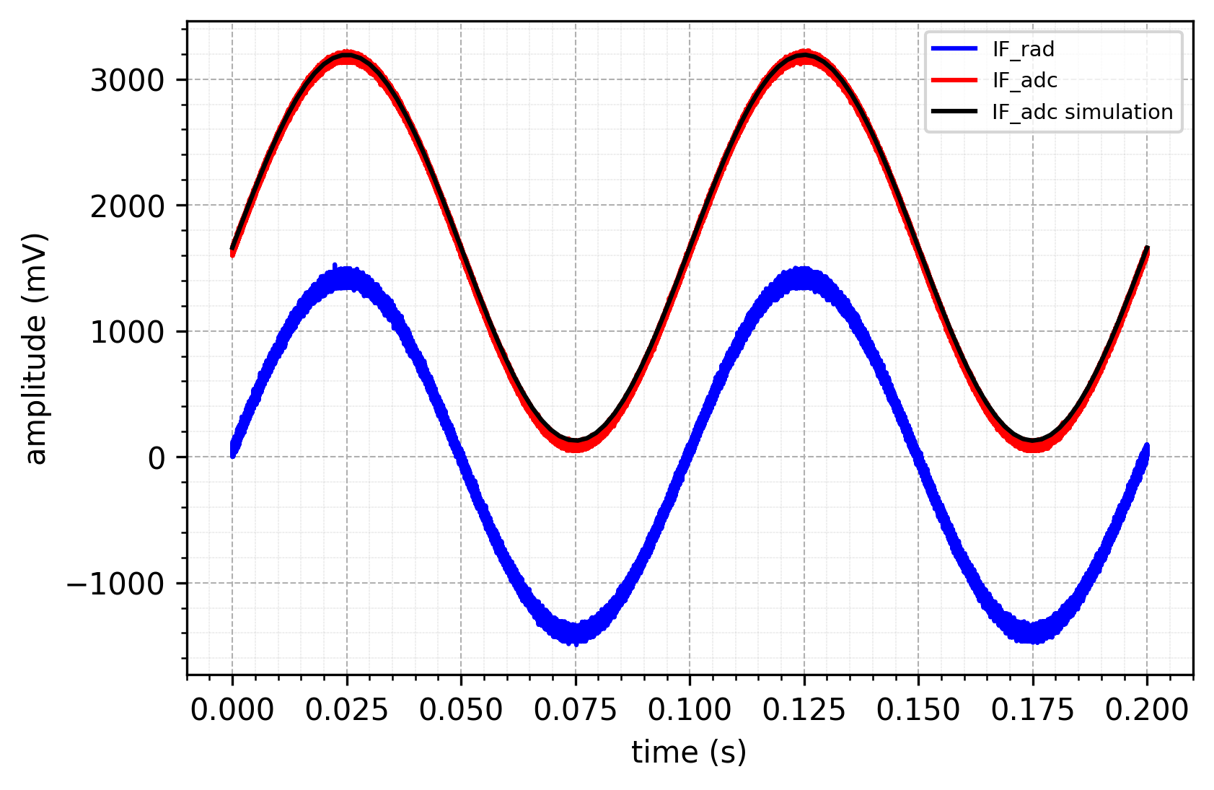
\includegraphics[width=0.7\linewidth]{sucio_graficos/if/10hz.png}
	\caption{Sin 10 Hz}
	\label{fig:moduloaprox50cmplancha}
\end{figure}
\begin{figure}[ht]
	\centering
	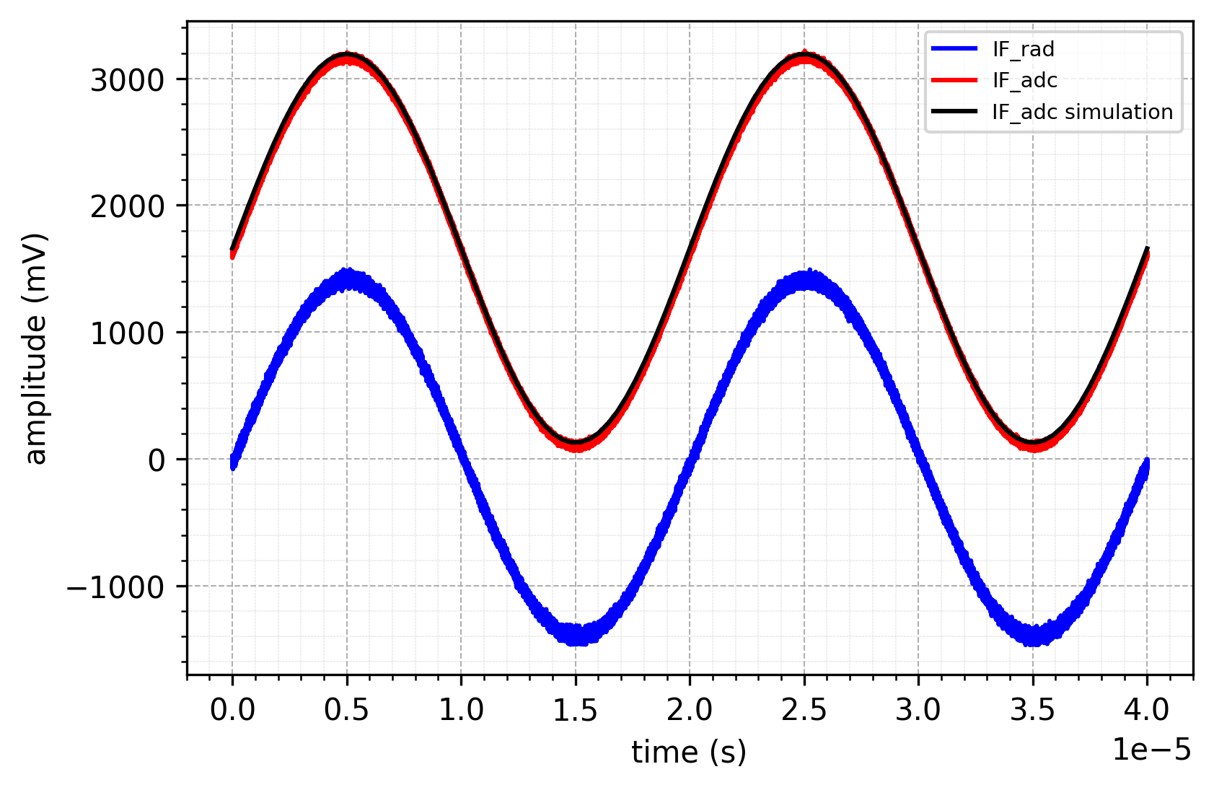
\includegraphics[width=0.7\linewidth]{sucio_graficos/if/50khz.png}
	\caption{Sin 50 kHz}
	\label{fig:moduloaprox50cmplancha}
\end{figure}
\begin{figure}[ht]
	\centering
	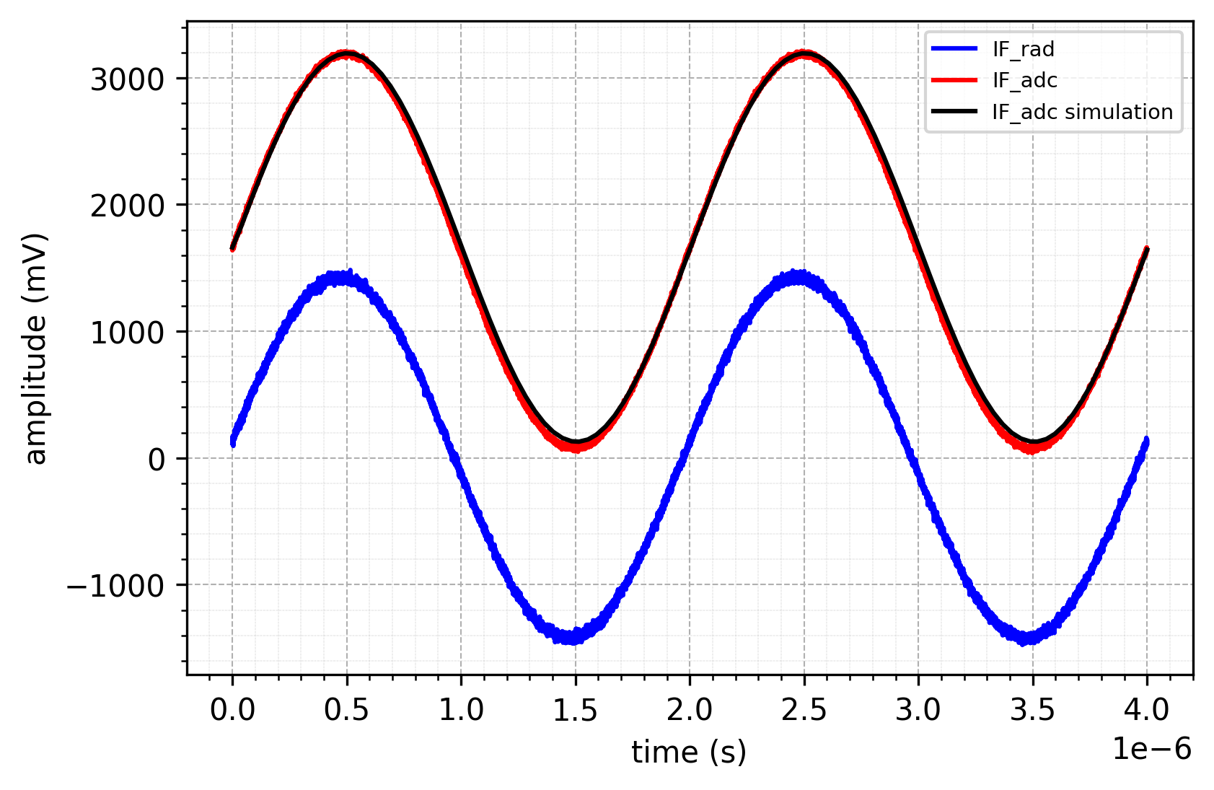
\includegraphics[width=0.7\linewidth]{sucio_graficos/if/500khz.png}
	\caption{Sin 500 kHz}
	\label{fig:moduloaprox50cmplancha}
\end{figure}
\begin{figure}[ht]
	\centering
	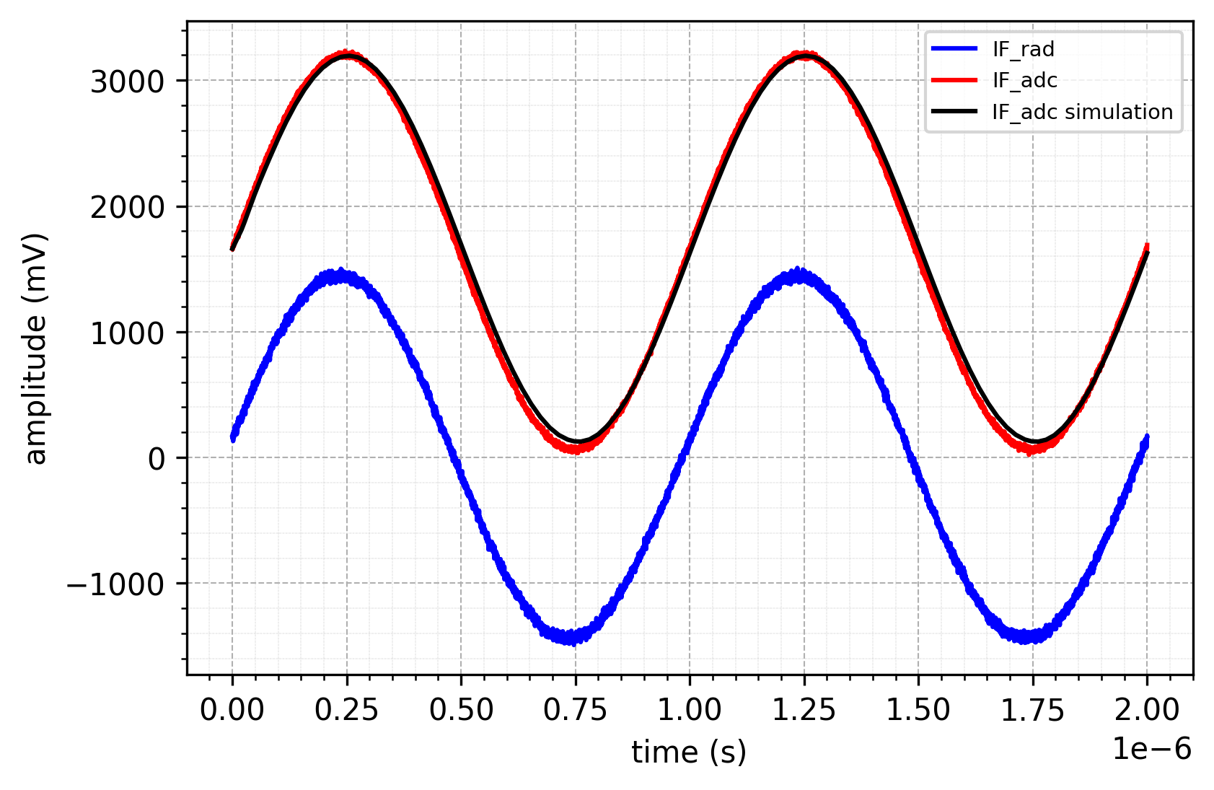
\includegraphics[width=0.7\linewidth]{sucio_graficos/if/1mhz.png}
	\caption{Sin 1 MHz}
	\label{fig:moduloaprox50cmplancha}
\end{figure}

\subsection{Digital signal processing}
\unsure[inline]{Tengo que centrarme aquí más en la parte del pipeline de procesado (tengo que redactar microdoppler mode junto con la documentación del sistema), sacar esto del dsp\_chain.md}
\subsection{Wireless communication}
\unsure[inline]{Tengo que centrarme aquí más en la parte del pipeline de procesado (tengo que redactar microdoppler mode junto con la documentación del sistema), tramas, etc, hablar de protocolos y comparación de protocolos wireless (ble al final mejor por compatibilidad, y consumo energético)}

\begin{figure}[ht]
	\centering
	\subfloat[Bottom view]{\includegraphics[width=0.5\linewidth]{img/radar_pcb_bot.png} \label{fig_cwlfm_ramps_freq}}
	\subfloat[Top view]{\includegraphics[width=0.49\linewidth]{img/radar_pcb_top.png} \label{fig_cwlfm_diff}}
	\todo[inline]{TODO: Change this layout for a diagram of necessary parts of a baseband board, leave this layout for our implementation}
	\caption{Views of a manufactured PCB featuring an example layout of the baseband stage reference design \label{fig:bb_board}}
\end{figure}

\chapter{Characterisation of the radar node}
\section{IF stage characterisation}
Aquí van las medidas del powerpoint redactadas:
\begin{itemize}
	\item Simulaciones de señales IF en el rango de tensiones y frecuencias
	\item Medidas de señales IF en el rango de tensiones y frecuencias
	\item Respuesta en frecuencia, simulación del TINA: bode\_plot.tiff y explicar que cubre el ancho de banda de las señales en banda base.
	\item Respuesta en frecuencia, medidas bode manual: del bodeplot del matplotlib y explicar que cubre el ancho de banda de las señales en banda base, y que es similar a la simulación
\end{itemize}

\section{ADC characterisation}
Aquí van las medidas del powerpoint redactadas, sobre el ADC:
\begin{itemize}
	\item Ruido de fondo del ADC. En tensiones y en dB.
	\item Simulación de adquisición del ADC del MCU: medidas adc\_sampling.staertsim3, sacar esto a .csv y poner plots
	\item Medidas de adquisición del ADC del MCU: medidas adc\_iq\_raw.hex de la memoria del micro, poner y explicar los gráficos del python
\end{itemize}
\begin{figure}[ht]
	\centering
	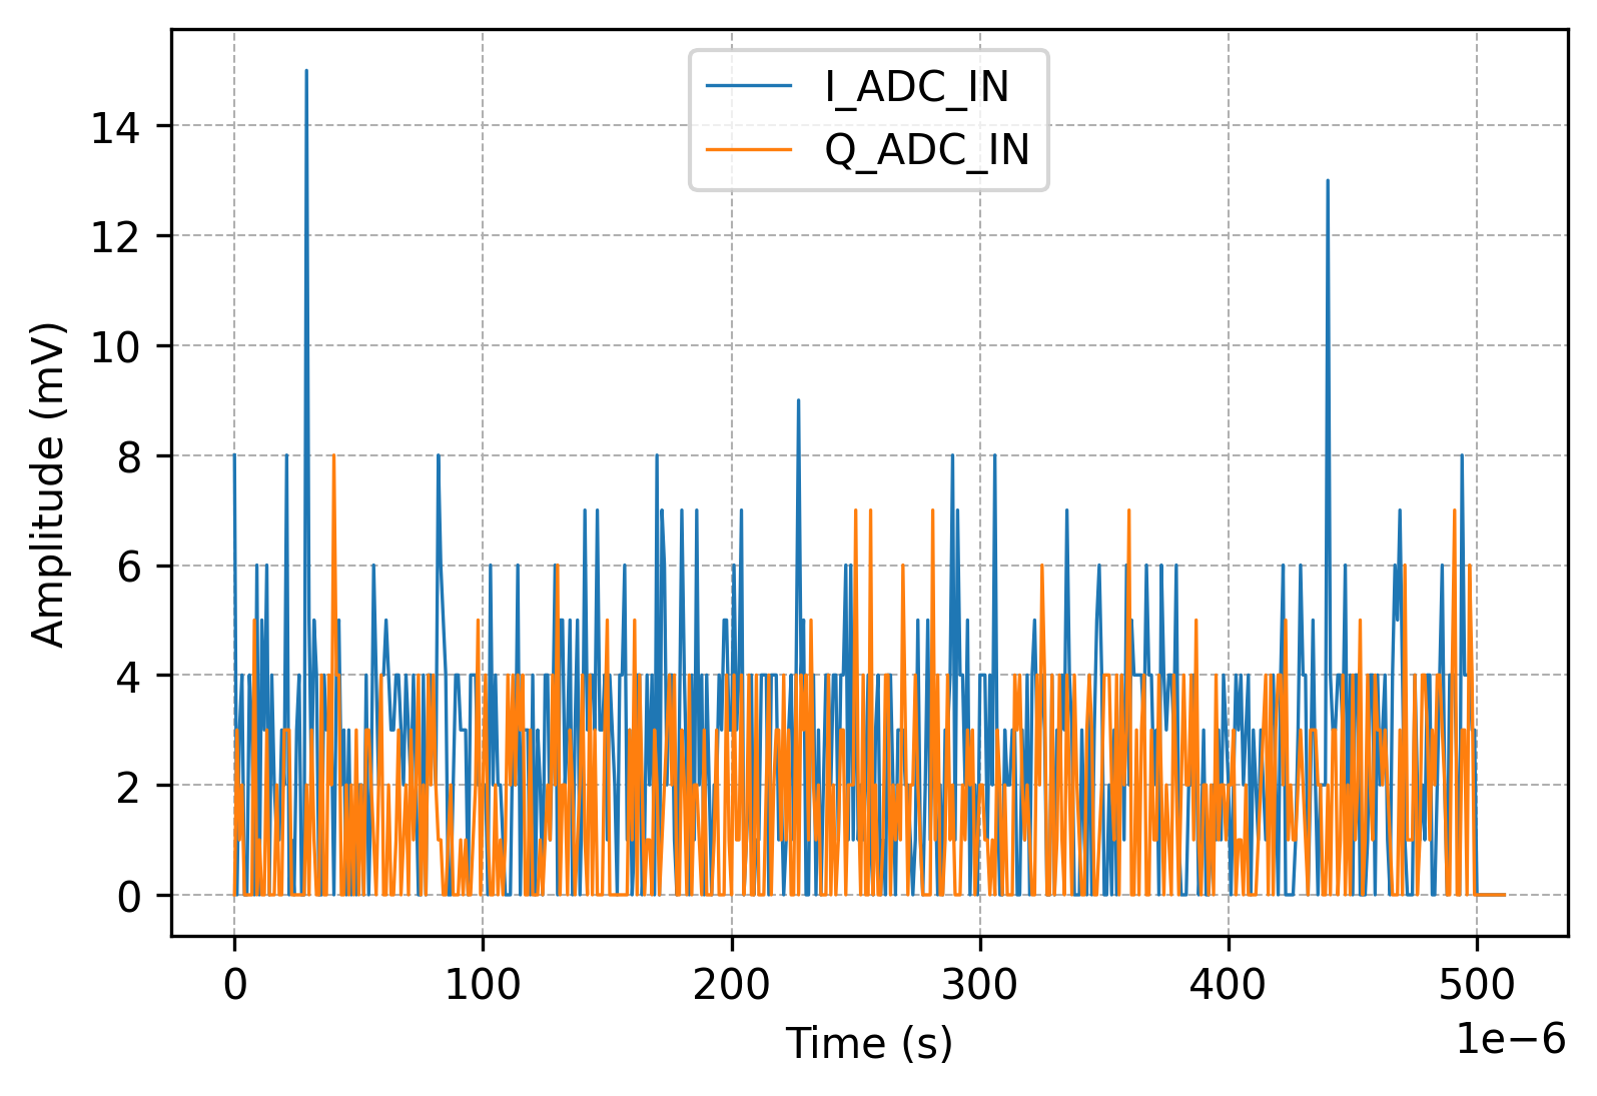
\includegraphics[width=0.7\linewidth]{sucio_graficos/adc/nf_mv.png}
	\caption{Noise Floor in mV}
	\label{fig:moduloaprox50cmplancha}
\end{figure}
\begin{figure}[ht]
	\centering
	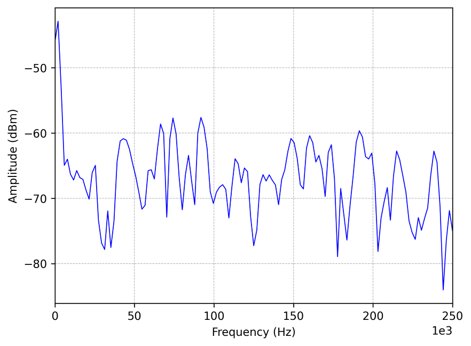
\includegraphics[width=0.7\linewidth]{sucio_graficos/adc/nf_dbm.png}
	\caption{Noise Floor in dBm}
	\label{fig:moduloaprox50cmplancha}
\end{figure}
\section{DSP Characterisation}
Aquí van las medidas del python redactadas, sobre el DSP pipeline:
\begin{itemize}
	\item Conversión a coma fija, explicar gráfico del error: conv\_q15\_error.eps y concluir que el error es menor del 1\% del rango de entrada del ADC, por lo que guay.
	\item Conversión a coma fija, ejemplos de medidas reales, del memdump adc\_iq\_q15.hex
\end{itemize}
\section{Wireless stack Characterisation}
Aquí van las medidas del python redactadas, sobre el BLE:
\begin{itemize}
	\item Caracterización binary throughput
	\item Caracterización BER
	\item Caracterización Ramp Lost Ratio to Distance
\end{itemize}


\unsure[inline]{Medida de la ecuación radar}
% el problema requiere el uso de radares cwlfm que son compactos, eficientes en coste y de bajo consumo

% establecer las condiciones de operación para las pruebas, requisitos radar/comunicaciones, hablar de anchos de banda, bitrate, etc. caracterización de las señales de frecuencia intermedia.

% adaptación hardware, creación sistema hardware,
%		hablar de mcu, seleccion mcu debido a qué criterios. hablar del adc del mcu
%		diseño de etapa if para adaptar el nivel de la señal.
%		desarrollo del pipeline de procesado digital de señal
%		desarrollo del pipeline de transmisión bluetooth
%		desarrollo de aplicación pc

% otro chapter
%		caracterización de las distintas partes

